\chapter{CodeSurfer}

\section{Usage}
CodeSurfer performs deep semantic analysis on the given code allowing the develper to understand how exactly the program works. It provides only valid executions.
Paths can be explored through a GUI and are and can be influenced by dependences (inter-variable assignments) including pointers, and allows automatic queries to resolve variables relationship. \cite{csurfUserGuide2012}

\begin{itemize}
	\itembf{String Constant Pointer Targets} (one-string/many-strings): differences in strings can be ignored (e.g. can be useful when analyzing GUI code) , or considered as different 
	\itembf{Variable Use/Def Sets} (yes/no): distinguish or not conditional kills 
	\itembf{Compute GMOD}(yes/no): determine dependences on non-local variables, this function is time-consuming
	\itembf{Compute Data Dependence}(yes/no): compute data dependency 
	\itembf{Compute Control Dependence} (yes/no):compute call dependecy, is only space consuming
	\itembf{Compute Summary Edges}(yes/no): is space and time consuming, it affects the interprocedural precision of slicing and chopping
	\itembf{Control Flow Edges}(yes/both/no): can compute CF edges, directed edges or none. The procedure is very cheap.
\end{itemize}

CodeSurefer can be run with 5 presets (super-lite, lite, medium, high and highest) they respectively enaable: nothing expensive, CFG only, no DD and imprecise pointer analysis, no context sensitive and string and fields are represented as scalar, finally no limitation is enforced. Lite and super-lite are intended as a check before the usage of a more precise execution.

\subsection{C++ Tutorial}
\subsubsection{Build a project}
Csurf gets a source code as input and build it generating a project that will be opened in the GUI. A project name, a compiler (or make if a makeFile is available) and a target has to be specified.
\begin{lstlisting}[language=bash]
csurf hook-start <projectName> <compiler> <target>

csurf hook-start hello cc hello.c

#WARN: instructions above will build the project with the lowest preset which does not allow some kind of analysis! To specify another level (e.g. highest) use command below:

csurf hook-start <projectName> -preset-build-options highest --- make  <target>
\end{lstlisting}

\subsubsection{Surfing a project}
A project can be opened using the project name without any extension.
\begin{lstlisting}
csurf <projectName>
\end{lstlisting}
clicking on the "source.c" element the code structure can be explored. CodeSurfer generates several functions such as \#zFile\_Initialization \#Global\_Initialization\_i (where i is a number).


\subsubsection{Queries}
The deep structure of a project is represented as a directed graph of program points connected by dependence edges. There are two main methods to calculate the dependes of a piece of code from the others:
\begin{itemize}
	\itembf{Data Dependeces:} is based on the assignment of values, a variables depends on others whose are involved in the calculation of its value. E.g. $x = y + z$ where x depends both on y and z.
	\itembf{Control Dependences:} the analysis is based on the control flow of the program (loops, conditions etc...), in this case the value of a variable depends on the variable present in the condition e.g. $if (x < 1) then (y = z) else (y = 0)$ in this case y depends on x.
\end{itemize}
Usually both CD and DD analysis are performed because the real value of a variable depends both on control flow and assignaments. In particular cases, to save resources, only one of the two analysis can be performed. In any case the result is not a final value but a flow graph which includes all variable dependences.\\
A Criterion is define as the combination of a point (a statement, line of code) and a specific variable, however CodeSurfer allows the usage of only the variable or the statment to define a criterion.
\\\\
CodeSurfer assumes that every loop may execute zero times, even when the program is simple enough to tell otherwise. In some contexts, all dependences are classified as either control or data dependences. In such contexts, declaration dependences are treated as data dependences.

\begin{itemize}
	\itembf{Predecessor/Successor:} starts from some query-points, pred/succ can be calculated DD and/or CD
	\itembf{BackWard/Forward Slicing:} the program is analyzed using CD and DD startring from the specified point and finding all the variables which contributes to the selected variable (Backward)or all the variables which the selected variable contributes to (Forward). Expanding the source file and clicking on a specific function Slicing can be applied: all reachable functions are coloured red, unreachable black. CodeSurfer typically errs on the safe side, creating false positives rather than missing effects that may be important.
	\itembf{Chop:} two points (chop-source and chop-target), the procedu is similar to the intersection of forward and backward slicing, the graph involves all operations that lead from the source to the targes. Source and target can be sets of points. 
\end{itemize}

The analysis of a program which involves functions is slightly complicated: suppose to have a function $int f(x)$ which is called in two points of the main(). When the function is called the main program stops esecutin, pass a value to f which returns a value, then the main restart executing. Analizing a code which calls two times the same function the resulting graph will have two edges from main to f and two edges from f to main. Obviously use the first main-to-f and the second f-to-main makes no sense and those spurious path have to be ignored.

%%%%%%%%%%%%%%%%%%%%%%%%%%%%%%%%%%%%%%%%%%%%%%%%%%%%%%%%%%%%%%%%%%%%%%%%%%%%%%%%%%%

\section{Program Representation}
\subsection{Control Flow Graph}
A CFG is a graph wich represent the executions steps of a program, it has only and entry point (where the execution begins) and only one exit point (where the execution ends). If the program has more than one entry/exit points them are merged in a single bogous entry/exit point. Each function is represented as a sub-CFG with the same characteristics.
\subsubsection{Syntax}
Inter-procedural edges (function call and return) are represented with an horizontal dashed arrow, while intra-procedural (inside the same function) steps are represented using a solid arrow. A vertical dotted line represent intraprocedural execution while a function is executed (i.e. the execution in main between call f and return f).
\begin{itemize}
	\itembf{IF} statments have labeled branches (true/false), the two branches merge once complethed the different execution
	\itembf{LOOPS} for and while statments have labeled branches (true/false), the  true branch execute the loop and return to the condition, the false branch skip the condition and reach the external code
	\itembf{EXCEPTION} are handled using a normal-exit vertex and an exceptional-exit vertex, both reach the exit status
\end{itemize}

\subsection{System Dependence Graph}
An SDG is similar to a CFG: it has a single entry/exit point so has it's functions, each instruction is a node and each step is an edge.
In addition to inter/intra-procedural edges SDGs introduce the Control and Data Dependences as seen above. Inter and intra procedural calls are still represented using dashed and solid edges, while the CD and DD are distinguished changing the colour of the (solid or dashed) edge.\\
Data Dependences are calculated using forward slicing, i.e. as the current variable will influence next states.
\begin{figure}
	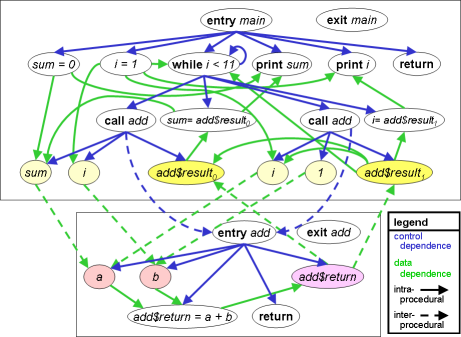
\includegraphics[ width=0.8 \linewidth]{./img/sdg_diagram.png}
	\caption{System Dependence Graph in CodeSurfer manual }
	\label{sdg_csurf}
\end{figure}



%%%%%%%%%%%%%%%%%%%%%%%%%%%%%%%%%%%%%%%%%%%%%%%%%%%%%%%%%%%%%%%%%%%%%%%%%%%%%%%%%%%

\section{Scheme}
Csurf can be extended both with c and shceme script. Scheme script can be run in batch mode and can access csur API in order to perform custum analisis. Those scripts can be run using 
\begin{lstlisting}
csurf -nogui -l <script.stk> <project>
\end{lstlisting}
Where nogui suppress the graphical interface and -l specify the script.
\\\\
Scheme is a functional language derived from Lisp, it is weakly typed and objects can be unlimited extended because the memory is managed internally.
\cite{abelson1991revised}
\subsection{Syntax}

Each expression has to be surrounded by parenthesis e.g. (display "hello world"), be aware that () are not intended like {} in C or Java but means something like "evaluate" as \$() does in bash. For this reason their number is relevant, for example (display "hello") is correct while ((display "hello")) is not!
Functions do not use the traditional parenthesized notation f(a, b) but are red in order from left to right where the first argument is the procedure (f a b). E.g. (a + b) is not valid, it has to be written as (+ a b)\\
Upper and lower case forms of a letter are never distin-guished except within character and string constants.\\

\subsubsection{Basic commands}
\begin{itemize}
	\itembf{;} comments are intruduced using ; and involves a single line
	\itembf{procedure?} conventionally are procedures which returns a boolean variable
	\itembf{procedure!} conventionally are procedures which write a result into a previously allocated memory location
	\itembf{"string"} strings are surrounded by "
	\itembf{lambda((args) (expr) values)} declares a procedure e.g. ((lambda (x y) (+ x y)) 3 4) returns 7 
	\itembf{define name (lambda)} without values associates a procedure to a name, it can be called using (name values)
	\itembf{let name ((var value))(expr)} is used to declare one or more variables which exists only inside the let scope, e.g. (let ((x 3) (y 4)) (+ x y)) returns 7. Nested let can hide variables declared in external scopes, on the contrary let* override the value of the external variable. The "name" parameter is optional: if it is specified the named let can be used like a local function.
	\itembf{cond(((test1)(inst1))((test2)(instr2)))} conditions are tested in succession, if one is satisfied the associated instruction is executed and following conditions are not tested. It basically works like a switch-case, the default condition can be simulated using (\#t (defaultop))
	\itembf{if (cond) (thenInstr)(elseInstr)} the condition is evaluated and, if it is satisfied, the first instruction has been executed, otherwise the second
	\itembf{set! var } 
\end{itemize}

\subsubsection{Reserved Keywords}
\begin{lstlisting} [language=lisp]
=>		do		or		and		else	quasiquote	begin	if		quote	case lambda	set!	cond	let		unquote	define	let*	unquote-splicing	delay	letrec
\end{lstlisting}

\subsubsection{Types}
	\begin{itemize}
		\itembf{Boolean} \#t \#f are the true and false values
		\itembf{Pairs} are represented with a dotted notation (a . b) that can be produced using the instruction (cons a b), car returns the first element, cdr the second. Be aware that cons (1 (list 2 3 4)) will return a list (1 2 3 4) and not a couple (1 . (2 3 4)) because is considered a special case of a list. In general the usage of cons should be avoided.
		\itembf{List} can be defined as a recursive applicarion of couples where the last element is null, for this reason car returns the first element and cdr the last one. a list can be declared using (list e1 e2 e3 ... en). Has some extra feture respect to pairs/nested pairs.
	\end{itemize}
	
\subsubsection{Constants}
	\begin{itemize}
		\itembf{'a} single quote, char value (a)
		\itembf{} backquote almost-constant data
		\itembf{"foo"} string, \ is the escape value
		\itembf{\#\textbackslash} character constants
		\itembf{\#()} vector constant
		\itembf{\#t \#f} boolean TRUE and FALSE
	\end{itemize}
	
\subsection{Function definition}
Basic function examples
\begin{lstlisting}[language=lisp]
;this function computes the sum of two elements
(define sum
	(lambda(a b)
		(+ a b)
	)
)

;this function compute recursively the factorial
(define fact
	(lambda(n)
		(if (= n 0)
			1						; base case "then"
			(* n (fact (- n 1)))	; recursion "else"
		)))
\end{lstlisting}

\subsection{Let}
Nested Let example
\begin{lstlisting}
; Nested Let
(define (myf vertex)
	(if (> vertex 0)
		(let ((x 12)(z 10))
			(let ((y (+ z 3)))
				(av-displayln  (+ x z))		
			)
		)
	)
)
\end{lstlisting}

\newpage
\subsection{List operation}
List declaration
\begin{lstlisting}[language=lisp]
; Empty list
(define lst (list))

(define lst (list 1 2 3 4 ))

; Equivalent to above
; Last element HAS to be empty otherwise a pair (list.element) will be generated!
(define lst (cons 1 (cons 2 (cons 3 (cons 4 '())))))
\end{lstlisting}

Some useful list operation
\begin{itemize}
	\itembf{(append list1 list2)} concatenation, both element has to be list eventually empty (list ) or of lenth 1 (list elm).
	\itembf{(member element list)} say whether or not an element belongs to the list return return the cdr of the list from the element on if true, false otherwise
	\itembf{(reverse lst)} reverse the list
	\itembf{(length lst)} returns the lenght of the list
	\itembf{(list-tail lst k)} which returns all elements except the fist k 
	\itembf{(list-ref list k)} which return the kth element
	\itembf{(null? element)} return true is a list is empty
\end{itemize}

Sum all the elements of a list without using lambda on the contrary of the previous example. 
\begin{lstlisting}[language=lisp]
(define (vsum1 lst) 
	(
		if(< (length lst)  1)
			0
			(+ (car lst) (vsum (cdr lst)))
	)	
)
\end{lstlisting}

Implementation of the built-in function reverse. Note that append requires list arguments otherwise will fail. The same function implemented using \textit{cons} will build a serie of nested couples which are NOT equivalent to the reversed list: length cannot be applied and cdr will return only the last elements because the first element is a couple of couple (of couple...).
\begin{lstlisting}[language=lisp]
(define (rev lst)
	(if (null? lst)
			'()
			(append(rev (cdr lst)) (list (car lst)))
	))
\end{lstlisting}

\subsection{File operations}
The following code open a port to read the file "myfile.txt" and pass it to readFile. This function read the file char by char through a named let (loop is a mere label) which works like a recursive function loop(x). This workaround in required beacause each read-char moves the read pointer a char ahead so the usage of ()display read-char) will print only a character every two.
\begin{lstlisting}
(define (readFile input)
	(let loop ((x (read-char input)))
		(if (not (eof-object? x))
		(begin
			(display x)
			(loop (read-char input))
		))))

(call-with-input-file "myfile.txt" readFile)
\end{lstlisting}

A simpler way to convert a file into a string is the following:
\begin{lstlisting}
	(define str (port->string port))
	(display str)
\end{lstlisting}

The output is simpler:
\begin{lstlisting}
(define (printFile output)
	(display "hello, world" output)
)

(call-with-output-file "myout.txt" printFile)
\end{lstlisting}

\section{CodeSurfer Data Structure}
In Scheme API each program is organized in a tree-like structure:
\begin{itemize}
	\itembf{SDG} System Dependence Graph, is composed by PDGs. An SDG represent the whole structure of a program including all methods.
	\itembf{PDG} Procedure Dependence Graph, is composed by Vertexes and Edges. A PDG represents a single procedure structure, it can belongs to several kind: user-defined (standard user-written functions), library and several kind of system defined (...-initialization) usually identified by a \# before their name.
	\itembf{Vertex} correspond to a program point, i.e. a combination of statement and line of code. Also vertexes are distinguised by kind, more intresting are entry/exit which represent the beginning and the end of a function, and call-site which identify a call to a function. Other Kind represent for example arguments, expression etc...
	\itembf{Edge} connect two vertexes, can be both intra-procedural (within the same PDG) and inter-procedural (between different PDGs). An edge is constituited by a vertex, which represent its target, and a label.
\end{itemize}

In \ref{csurf_uml} can be seen a partial representation of the Code Surfer class diagram. Only most significative functions and classes have been included in this representation. Note that Scheme is not an object-oriented language: several functions have been represented using the "object.function()" which has to be interpreted as a function which gets the object itself i.e. "(function object)".
\begin{figure}
	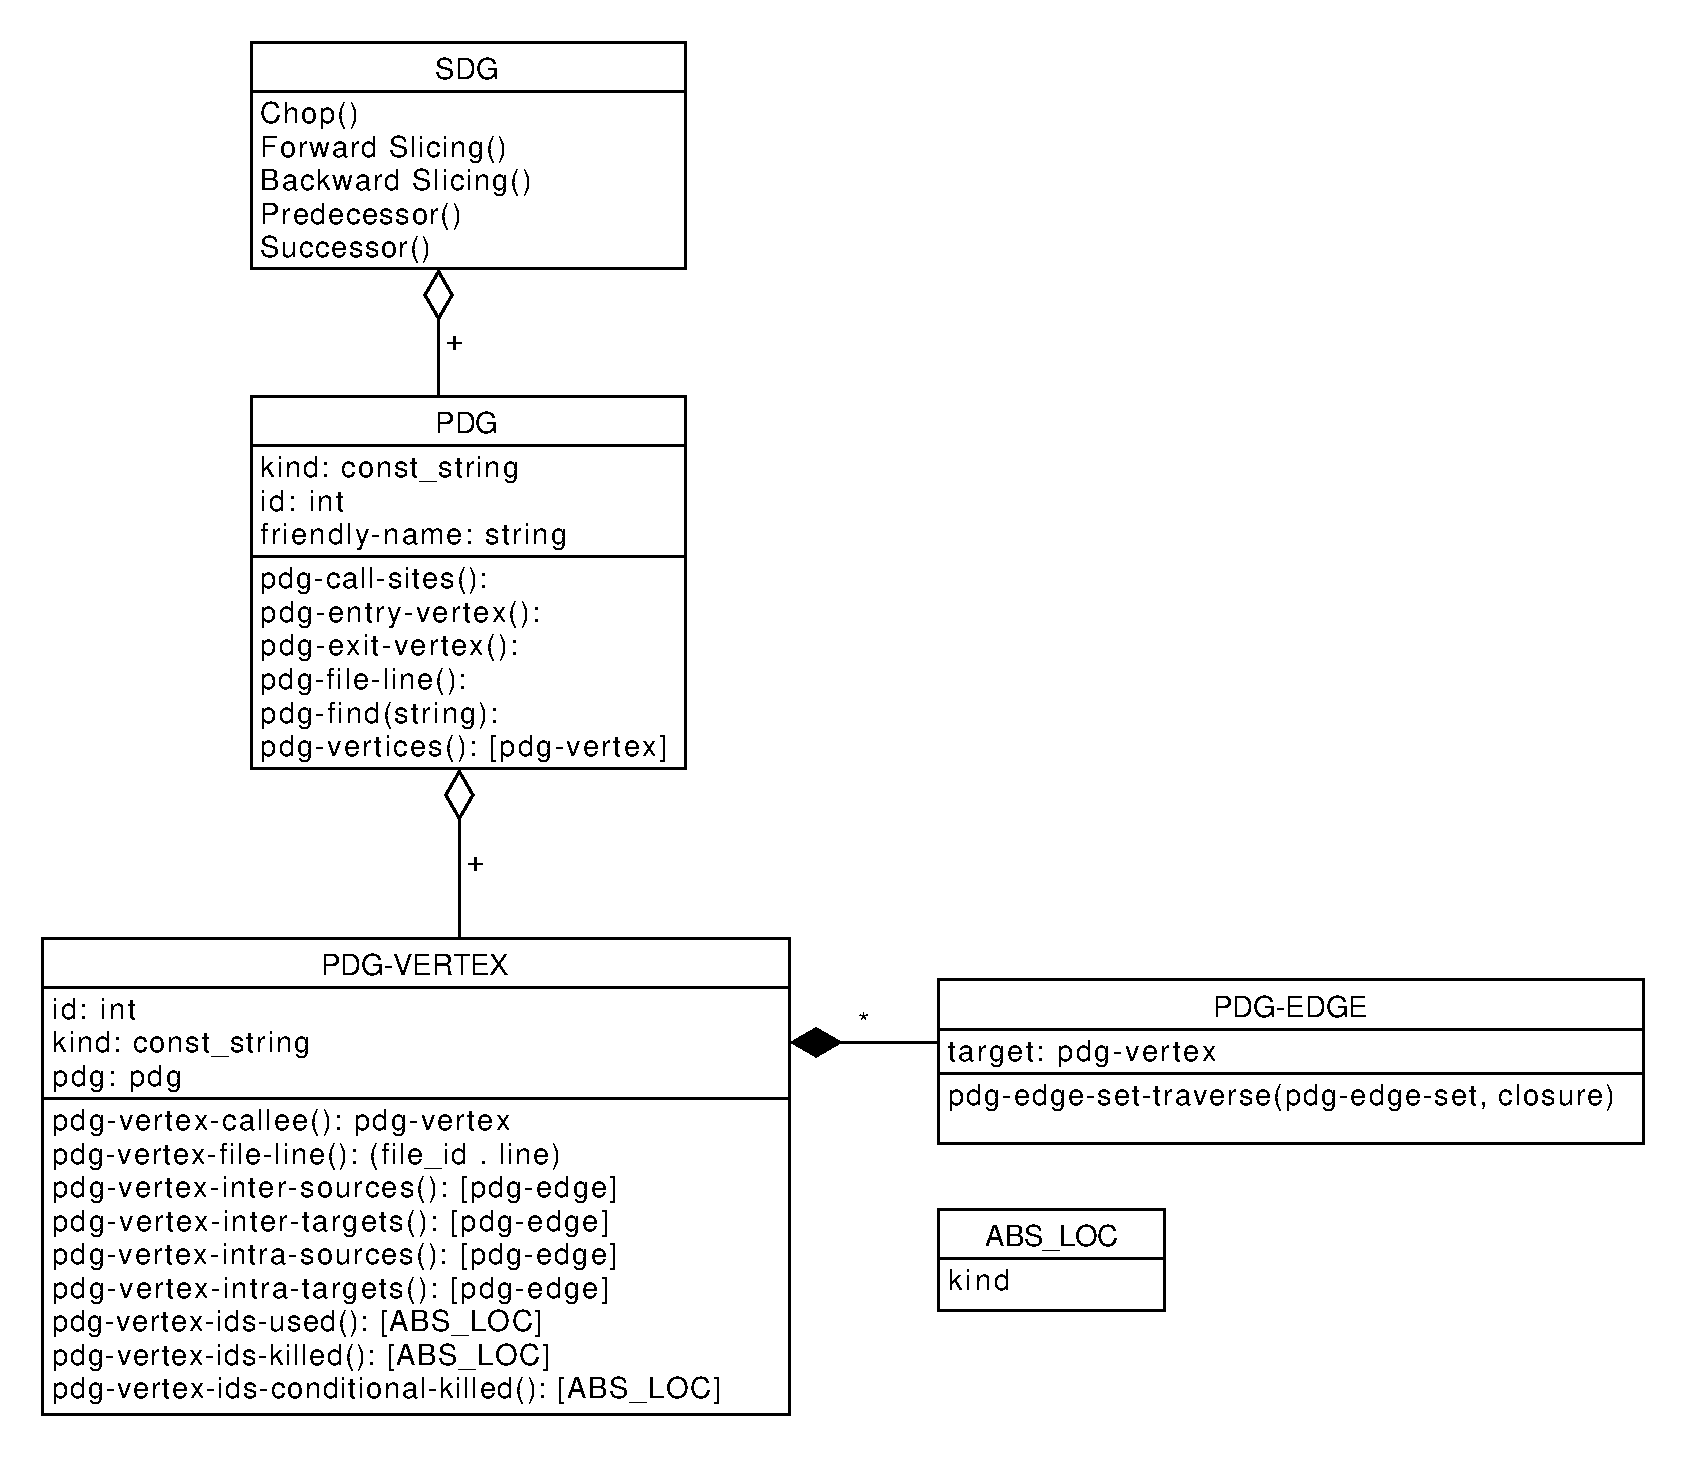
\includegraphics[ width=1.2 \linewidth]{./img/csurf_classdiagram.pdf}
	\caption{Code surfer data structure}
	\label{csurf_uml}
\end{figure}


\section{Data Distance}
The main point of distance graph can be summarized as follow: for a given pdg fin all its vertexes and for each vertex build a pair (used.killed) where:
\begin{itemize}
	\itembf{Used:} a program point where a variable is taken (i.e. read in some way). Can be used directly or indirectly is accessed using its pointer.
	
	\itembf{Killed:} a program point where the value contained in a variable is necessarily changed is a kill of that variable. A conditional kill is a kill bounded to a condition, so a c.k. may or may not happen.
\end{itemize}
Each couple represents a use-kill bound which is an edge in the graph, for example  $x = y +1$ corresponds to a pair (x.y).


\begin{figure}
	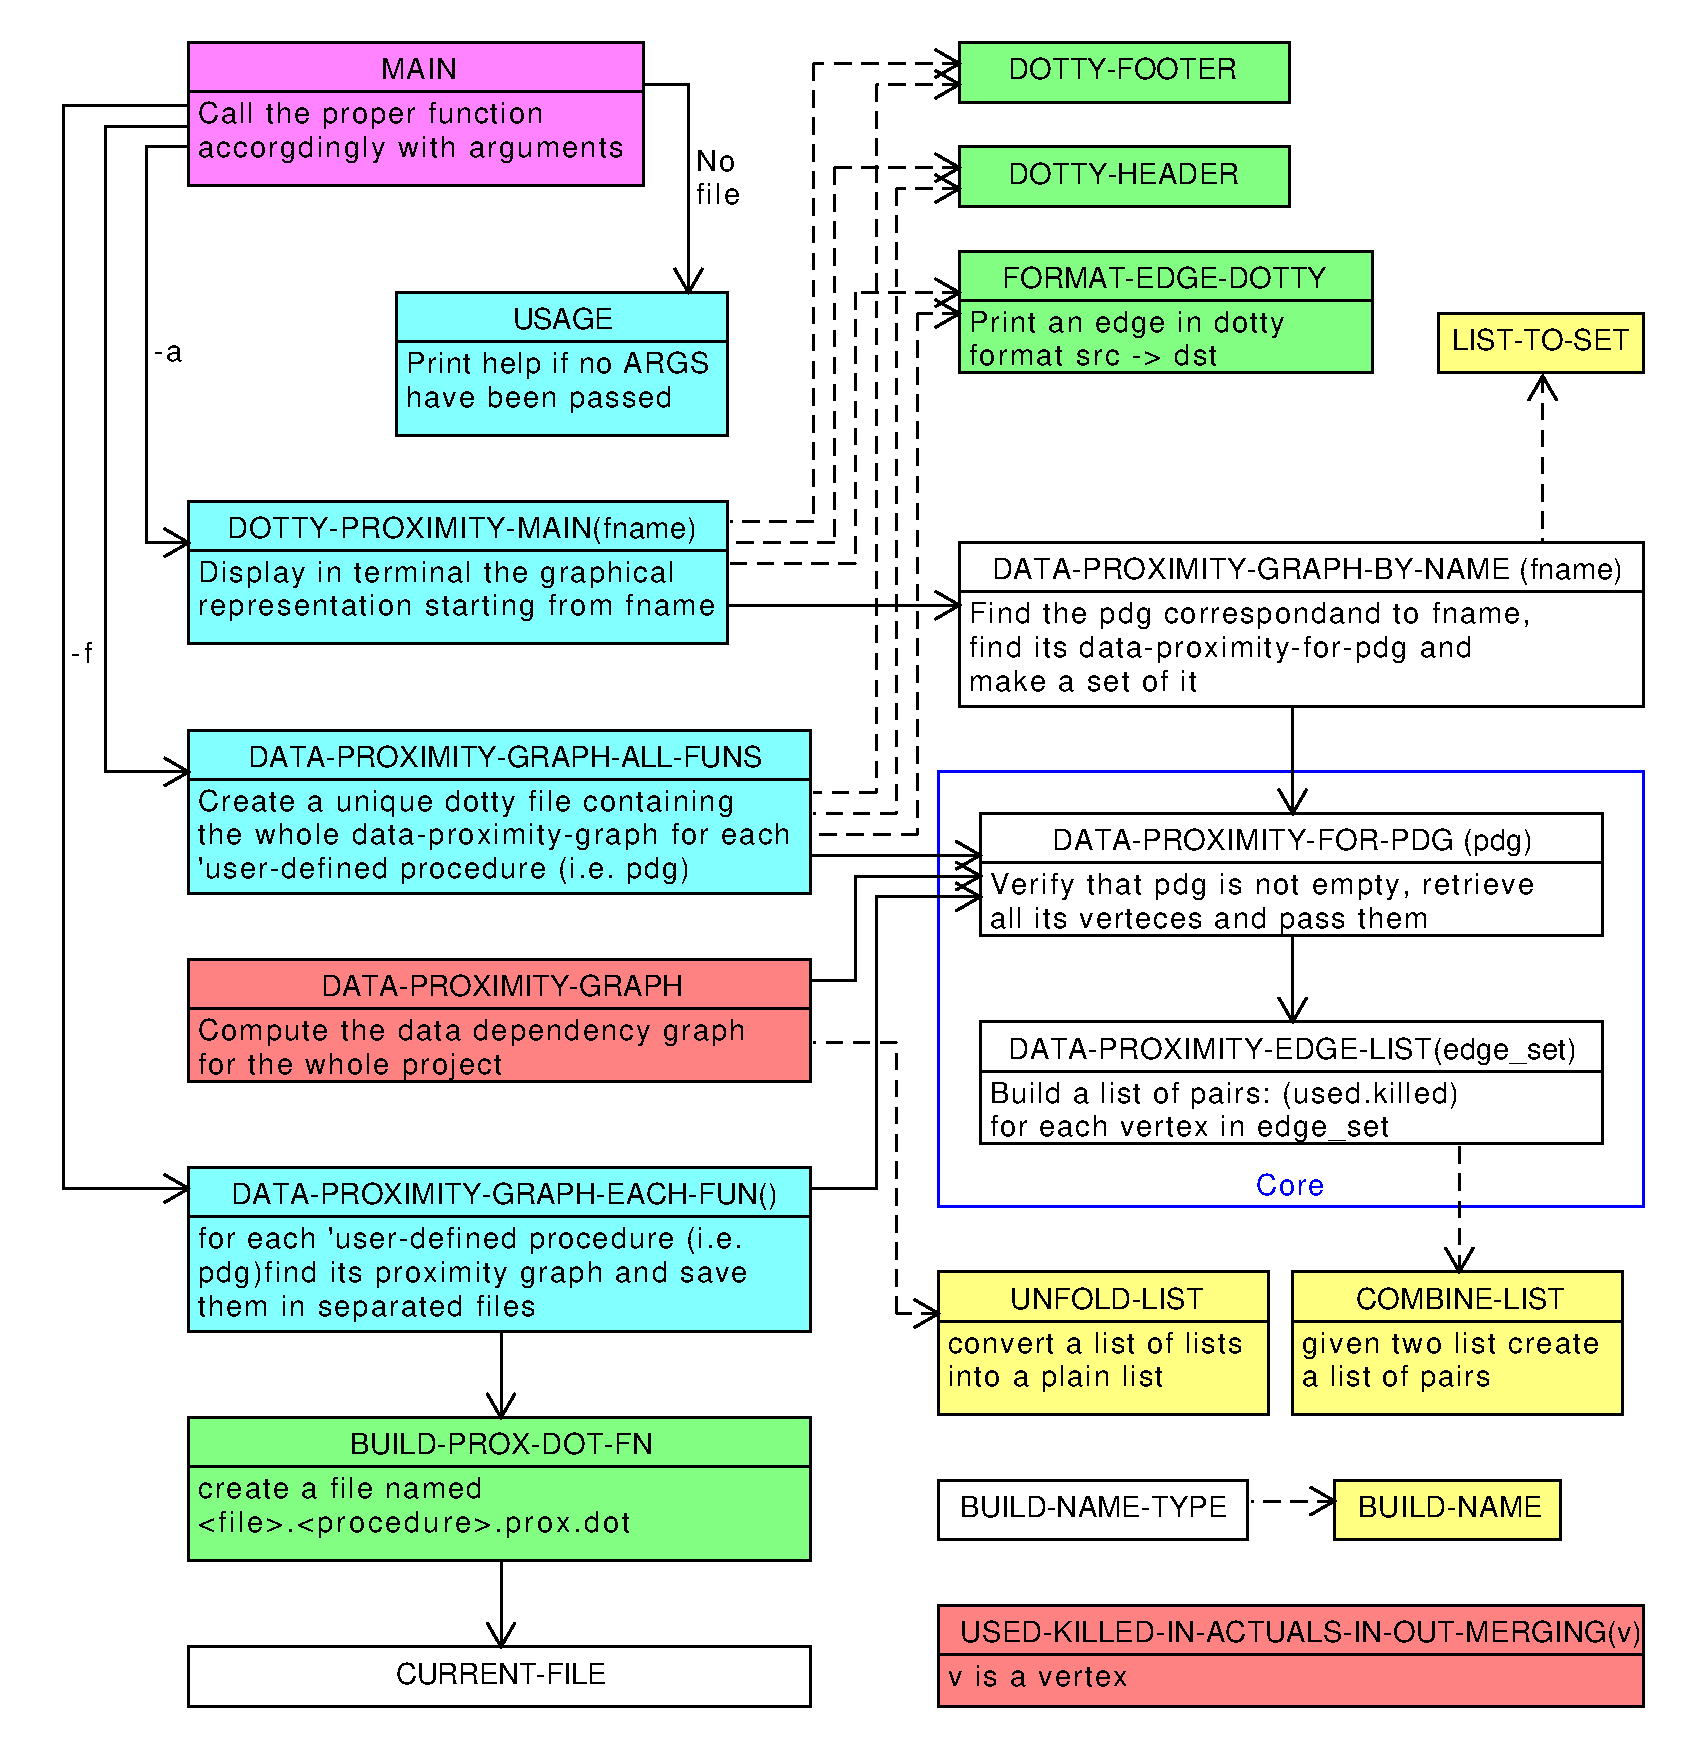
\includegraphics[ width=1 \linewidth]{./img/dd_descr_tree.pdf}
	\caption{Tiella's dd.stk program structure. Magenta represents main, cyan option args-dependent function, green output function (dotty support) and yellow are externally-defined functions.}
	\label{dd_uml}
\end{figure}

